% Options for packages loaded elsewhere
\PassOptionsToPackage{unicode}{hyperref}
\PassOptionsToPackage{hyphens}{url}
%
\documentclass[
  man]{apa6}
\usepackage{amsmath,amssymb}
\usepackage{lmodern}
\usepackage{iftex}
\ifPDFTeX
  \usepackage[T1]{fontenc}
  \usepackage[utf8]{inputenc}
  \usepackage{textcomp} % provide euro and other symbols
\else % if luatex or xetex
  \usepackage{unicode-math}
  \defaultfontfeatures{Scale=MatchLowercase}
  \defaultfontfeatures[\rmfamily]{Ligatures=TeX,Scale=1}
\fi
% Use upquote if available, for straight quotes in verbatim environments
\IfFileExists{upquote.sty}{\usepackage{upquote}}{}
\IfFileExists{microtype.sty}{% use microtype if available
  \usepackage[]{microtype}
  \UseMicrotypeSet[protrusion]{basicmath} % disable protrusion for tt fonts
}{}
\makeatletter
\@ifundefined{KOMAClassName}{% if non-KOMA class
  \IfFileExists{parskip.sty}{%
    \usepackage{parskip}
  }{% else
    \setlength{\parindent}{0pt}
    \setlength{\parskip}{6pt plus 2pt minus 1pt}}
}{% if KOMA class
  \KOMAoptions{parskip=half}}
\makeatother
\usepackage{xcolor}
\usepackage{graphicx}
\makeatletter
\def\maxwidth{\ifdim\Gin@nat@width>\linewidth\linewidth\else\Gin@nat@width\fi}
\def\maxheight{\ifdim\Gin@nat@height>\textheight\textheight\else\Gin@nat@height\fi}
\makeatother
% Scale images if necessary, so that they will not overflow the page
% margins by default, and it is still possible to overwrite the defaults
% using explicit options in \includegraphics[width, height, ...]{}
\setkeys{Gin}{width=\maxwidth,height=\maxheight,keepaspectratio}
% Set default figure placement to htbp
\makeatletter
\def\fps@figure{htbp}
\makeatother
\setlength{\emergencystretch}{3em} % prevent overfull lines
\providecommand{\tightlist}{%
  \setlength{\itemsep}{0pt}\setlength{\parskip}{0pt}}
\setcounter{secnumdepth}{-\maxdimen} % remove section numbering
% Make \paragraph and \subparagraph free-standing
\ifx\paragraph\undefined\else
  \let\oldparagraph\paragraph
  \renewcommand{\paragraph}[1]{\oldparagraph{#1}\mbox{}}
\fi
\ifx\subparagraph\undefined\else
  \let\oldsubparagraph\subparagraph
  \renewcommand{\subparagraph}[1]{\oldsubparagraph{#1}\mbox{}}
\fi
\newlength{\cslhangindent}
\setlength{\cslhangindent}{1.5em}
\newlength{\csllabelwidth}
\setlength{\csllabelwidth}{3em}
\newlength{\cslentryspacingunit} % times entry-spacing
\setlength{\cslentryspacingunit}{\parskip}
\newenvironment{CSLReferences}[2] % #1 hanging-ident, #2 entry spacing
 {% don't indent paragraphs
  \setlength{\parindent}{0pt}
  % turn on hanging indent if param 1 is 1
  \ifodd #1
  \let\oldpar\par
  \def\par{\hangindent=\cslhangindent\oldpar}
  \fi
  % set entry spacing
  \setlength{\parskip}{#2\cslentryspacingunit}
 }%
 {}
\usepackage{calc}
\newcommand{\CSLBlock}[1]{#1\hfill\break}
\newcommand{\CSLLeftMargin}[1]{\parbox[t]{\csllabelwidth}{#1}}
\newcommand{\CSLRightInline}[1]{\parbox[t]{\linewidth - \csllabelwidth}{#1}\break}
\newcommand{\CSLIndent}[1]{\hspace{\cslhangindent}#1}
\ifLuaTeX
\usepackage[bidi=basic]{babel}
\else
\usepackage[bidi=default]{babel}
\fi
\babelprovide[main,import]{english}
% get rid of language-specific shorthands (see #6817):
\let\LanguageShortHands\languageshorthands
\def\languageshorthands#1{}
% Manuscript styling
\usepackage{upgreek}
\captionsetup{font=singlespacing,justification=justified}

% Table formatting
\usepackage{longtable}
\usepackage{lscape}
% \usepackage[counterclockwise]{rotating}   % Landscape page setup for large tables
\usepackage{multirow}		% Table styling
\usepackage{tabularx}		% Control Column width
\usepackage[flushleft]{threeparttable}	% Allows for three part tables with a specified notes section
\usepackage{threeparttablex}            % Lets threeparttable work with longtable

% Create new environments so endfloat can handle them
% \newenvironment{ltable}
%   {\begin{landscape}\centering\begin{threeparttable}}
%   {\end{threeparttable}\end{landscape}}
\newenvironment{lltable}{\begin{landscape}\centering\begin{ThreePartTable}}{\end{ThreePartTable}\end{landscape}}

% Enables adjusting longtable caption width to table width
% Solution found at http://golatex.de/longtable-mit-caption-so-breit-wie-die-tabelle-t15767.html
\makeatletter
\newcommand\LastLTentrywidth{1em}
\newlength\longtablewidth
\setlength{\longtablewidth}{1in}
\newcommand{\getlongtablewidth}{\begingroup \ifcsname LT@\roman{LT@tables}\endcsname \global\longtablewidth=0pt \renewcommand{\LT@entry}[2]{\global\advance\longtablewidth by ##2\relax\gdef\LastLTentrywidth{##2}}\@nameuse{LT@\roman{LT@tables}} \fi \endgroup}

% \setlength{\parindent}{0.5in}
% \setlength{\parskip}{0pt plus 0pt minus 0pt}

% Overwrite redefinition of paragraph and subparagraph by the default LaTeX template
% See https://github.com/crsh/papaja/issues/292
\makeatletter
\renewcommand{\paragraph}{\@startsection{paragraph}{4}{\parindent}%
  {0\baselineskip \@plus 0.2ex \@minus 0.2ex}%
  {-1em}%
  {\normalfont\normalsize\bfseries\itshape\typesectitle}}

\renewcommand{\subparagraph}[1]{\@startsection{subparagraph}{5}{1em}%
  {0\baselineskip \@plus 0.2ex \@minus 0.2ex}%
  {-\z@\relax}%
  {\normalfont\normalsize\itshape\hspace{\parindent}{#1}\textit{\addperi}}{\relax}}
\makeatother

% \usepackage{etoolbox}
\makeatletter
\patchcmd{\HyOrg@maketitle}
  {\section{\normalfont\normalsize\abstractname}}
  {\section*{\normalfont\normalsize\abstractname}}
  {}{\typeout{Failed to patch abstract.}}
\patchcmd{\HyOrg@maketitle}
  {\section{\protect\normalfont{\@title}}}
  {\section*{\protect\normalfont{\@title}}}
  {}{\typeout{Failed to patch title.}}
\makeatother

\usepackage{xpatch}
\makeatletter
\xapptocmd\appendix
  {\xapptocmd\section
    {\addcontentsline{toc}{section}{\appendixname\ifoneappendix\else~\theappendix\fi\\: #1}}
    {}{\InnerPatchFailed}%
  }
{}{\PatchFailed}
\keywords{keywords\newline\indent Word count: X}
\DeclareDelayedFloatFlavor{ThreePartTable}{table}
\DeclareDelayedFloatFlavor{lltable}{table}
\DeclareDelayedFloatFlavor*{longtable}{table}
\makeatletter
\renewcommand{\efloat@iwrite}[1]{\immediate\expandafter\protected@write\csname efloat@post#1\endcsname{}}
\makeatother
\usepackage{lineno}

\linenumbers
\usepackage{csquotes}
\ifLuaTeX
  \usepackage{selnolig}  % disable illegal ligatures
\fi
\IfFileExists{bookmark.sty}{\usepackage{bookmark}}{\usepackage{hyperref}}
\IfFileExists{xurl.sty}{\usepackage{xurl}}{} % add URL line breaks if available
\urlstyle{same} % disable monospaced font for URLs
\hypersetup{
  pdftitle={The title},
  pdfauthor={First Author1 \& Ernst-August Doelle1,2},
  pdflang={en-EN},
  pdfkeywords={keywords},
  hidelinks,
  pdfcreator={LaTeX via pandoc}}

\title{The title}
\author{First Author\textsuperscript{1} \& Ernst-August Doelle\textsuperscript{1,2}}
\date{}


\shorttitle{Title}

\authornote{

Add complete departmental affiliations for each author here. Each new line herein must be indented, like this line.

Enter author note here.

The authors made the following contributions. First Author: Conceptualization, Writing - Original Draft Preparation, Writing - Review \& Editing; Ernst-August Doelle: Writing - Review \& Editing, Supervision.

Correspondence concerning this article should be addressed to First Author, Postal address. E-mail: \href{mailto:my@email.com}{\nolinkurl{my@email.com}}

}

\affiliation{\vspace{0.5cm}\textsuperscript{1} Wilhelm-Wundt-University\\\textsuperscript{2} Konstanz Business School}

\abstract{%
One or two sentences providing a \textbf{basic introduction} to the field, comprehensible to a scientist in any discipline.

Two to three sentences of \textbf{more detailed background}, comprehensible to scientists in related disciplines.

One sentence clearly stating the \textbf{general problem} being addressed by this particular study.

One sentence summarizing the main result (with the words ``\textbf{here we show}'' or their equivalent).

Two or three sentences explaining what the \textbf{main result} reveals in direct comparison to what was thought to be the case previously, or how the main result adds to previous knowledge.

One or two sentences to put the results into a more \textbf{general context}.

Two or three sentences to provide a \textbf{broader perspective}, readily comprehensible to a scientist in any discipline.
}



\begin{document}
\maketitle

\hypertarget{the-current-research}{%
\section{The Current Research}\label{the-current-research}}

Our primary prediction is that a cognitive load manipulation will inhibit people's ability to provide reasons for their judgment, leading to greater habitual responses (either dumbfounding or nothing wrong or both). We present a pre-registered study to test this prediction of a conflict in dual-process explanation of moral dumbfounding. We experimentally manipulated cognitive load, and predicted that this cognitive load manipulation will inhibit people's ability to provide reasons for their judgment, leading to greater habitual responses (either nothing wrong or dumbfounding or both).

Our cognitive load manipulation involved a secondary task requiring participants to pay attention to a stream of numbers on the screen while completing the moral judgment task. We conducted a series of pilot studies (see Supplement Studies S1 - S5) involving two different memory tasks. The effectiveness of these memory tasks in manipulating cognitive load was unclear, and it is possible that participants could cheat on these memory tasks (particularly for online samples). As such, we selected a cognitive load manipulation that required participants to pay attention to a secondary task (rather than a memory task) while engaged in the primary judgment task (in line with Greene, Morelli, Lowenberg, Nystrom, \& Cohen, 2008).

The data for this study (and all pilot studies), as well as the analysis code for all studies, and full materials for this study including jsPsych script are publicly available at \color{blue}\url{https://osf.io/fcd5r/?view_only=9fb6e506e53340c189b98453bb2b6eaf}\color{black}. This study was pre-registered and the pre-registration is available at \color{blue}\url{https://aspredicted.org/XZP_UHW}\color{black}. All analyses were conducted in R (R Core Team, 2021), see analysis code for full list of packages.

\hypertarget{method}{%
\subsection{Method}\label{method}}

\hypertarget{participants-and-design}{%
\subsubsection{Participants and design}\label{participants-and-design}}

This study was a between subjects design. The dependent variable was rates of reason-giving/dumbfounding (measured using the critical slide with 3 response options: 1: reason-giving; 2: nothing-wrong; 3: dumbfounded response - admission). The primary independent variable was cognitive load with two levels: present and absent. To manipulate cognitive load, a stream of numbers scrolled across the screen above the question text, and participants were required to pay attention to how many times they saw a given number. The scenario served as a secondary independent variable, we used four scenarios: \emph{Julie and Mark (Incest)}, \emph{Jennifer (Cannibal)}, \emph{Trolley}, \emph{Heinz} (see Supplementary Materials for full text of each).

A total sample of 1899 participants (984 female, 876 male, 17 non-binary, 1 other, 5 prefer not to say; \emph{M}\textsubscript{age} = 43.22, min = 18, max = 84, \emph{SD} = 15.85) started the survey. Participants in this sample were recruited from Prolific (\emph{n\textsubscript{UK}} = 963, \emph{n\textsubscript{US}} = 936).\footnote{A priori power analysis indicated that, for the primary research question (the influence of cognitive load on dumbfounded responding), in order to detect a large effect size (\emph{V} = .35) with 80\% power, a sample of \emph{N} = 79 participants was required; in order to detect a medium effect size (\emph{V} = .21) with 80\% power a sample of \emph{N} = 218 participants was required; in order to detect a small effect size (\emph{V} = .07) with 80\% power a sample of \emph{N} = 1966 was required.}

Participants who failed both manipulation checks (\emph{n} = 7) or who had missing data for the measures of interest were removed, leaving a total sample of 1686 participants (867 female, 799 male, 14 non-binary, 1 other, 5 prefer not to say; \emph{M}\textsubscript{age} = 43.81, min = 18, max = 83, \emph{SD} = 15.76), \emph{n\textsubscript{UK}} = 842, \emph{n\textsubscript{US}} = 844.

\hypertarget{procedure-and-materials}{%
\subsubsection{Procedure and materials}\label{procedure-and-materials}}

Data were collected using an online questionnaire developed with \emph{jsPsych} and distributed with \emph{cognition.run}. Participants were presented with one of four moral scenarios (\emph{Julie and Mark}, \emph{Jennifer}, \emph{Trolley}, \emph{Heinz}, see supplementary materials for full wording), previously used in studies of moral dumbfounding (McHugh et al., 2017). Participants rated on a 7-point Likert scale how right or wrong the behavior of the character in the scenario was (where, 1 = \emph{Morally wrong}; 4 = \emph{neutral}; 7 = \emph{Morally right}), and were given an opportunity to provide reasons for their judgment. Following this, participants were presented with a series of counter-arguments, which refute commonly used justifications for rating the behavior as ``wrong'' (see supplementary materials for full text of scenarios and all counter-arguments).

Dumbfounding was measured using the critical slide (developed by McHugh et al., 2017). This contained a statement defending the behavior and a question as to how the behavior could be wrong (e.g., ``Julie and Mark's behavior did not harm anyone, how can there be anything wrong with what they did?''). There were three possible answer options: (a) ``It's wrong, and I can provide a valid reason'' (reasons); (b) ``It's wrong, but I can't think of a reason'' (an admission of not having reasons); (c) ``There is nothing wrong''. The order of these response options was randomized. Participants who selected (a) were prompted to type a reason. The selecting of an option (b), the admission of not having reasons, was taken to be a dumbfounded response.\footnote{This measure avoids the potential confounding influence of qualitative differences between different response types; that is, participants indicate whether they can provide reasons for their judgments or not, and this is our measure (not whether or not they actually provide reasons, as this different type of response would not be comparable to a dumbfounded response).}
We note that this measure provides a conservative measure of dumbfounded responding {[}see McHugh et al. (2017) for discussion). A key advantage of this measure of dumbfounding is its suitability for use with cognitive load manipulations. The task requirements for each of the three response options are qualitatively the same (selecting a response), eliminating the potential confounding influence of different types of task requirements. Importantly, participants who selected (a) were only prompted to provide a reason after their response to the critical slide had been submitted and recorded, and the survey had proceeded to the next page. Participants did not know they would be required to provide a reason prior to the presentation of this prompt.

We included a video stream of numbers scrolling above the question text for our cognitive load manipulation, drawing on Greene et al. (2008). The video was wide enough to display 3 numbers at a time, and the numbers scrolled past at a speed of 2 numbers per second. Participants were asked to attend to and report (on a subsequent page) how many times a particular number appeared in the stream, while answering the target question. Following an initial training task, the video was presented while participants made their initial judgments, while they responded to the critical slide, and while they were providing their revised judgments.

Two attention check tasks were included for all participants, these included a brief paragraph of text where instructions for the correct response were embedded within the text. The wording of the text was misleading such that if participants skimmed or only read some of the text they would likely provide an incorrect response.

Participants clicked on the survey link and were randomly assigned to either the experimental condition or the control condition, within which they were randomly presented with one of the four scenarios. The study was complete within 5 minutes.

\hypertarget{results}{%
\subsection{Results}\label{results}}

One thousand three hundred sixty-five participants (80.96\%) rated the behavior described as wrong initially, and one thousand three hundred forty three participants (79.66\%) rated the behavior as wrong at the end of the task. Initial ratings (\emph{M} = 2.26, \emph{SD} = 1.63) were significantly more severe than revised ratings (\emph{M} = 2.34, \emph{SD} = 1.66), \emph{t}(1685) = -2.69, \emph{p} = .007; \emph{d} = 0.07. Inspection of the binned judgments revealed that two hundred (11.86\%) participants changed the valence of their judgments, breakdown of the changes in judgments is in Table 16 (full sample) and Table 17 (by scenario) in the supplementary materials.

A 2 \(\times\) 2 factorial ANOVA revealed significant differences in initial judgments depending on both condition \emph{F}(1, 1678) = 26.65, \emph{p} \textless{} .001, partial \(\eta\)\textsuperscript{2} = .016, and scenario \emph{F}(3, 1678) = 69.30, \emph{p} \textless{} .001, partial \(\eta\)\textsuperscript{2} = .110. Participants under cognitive load were significantly (\emph{p} \textless{} .001) less harsh in their judgments (\emph{M} = 2.46, \emph{SD} = 1.75) than those in the control condition (\emph{M} = 2.07, \emph{SD} = 1.49). Participants rated \emph{Jennifer} as the most wrong (\emph{M} = 1.53, \emph{SD} = 1.13), followed by \emph{Julie and Mark} (\emph{M} = 2.05, \emph{SD} = 1.65, \emph{p} \textless{} .001), then \emph{Heinz} (\emph{M} = 2.49, \emph{SD} = 1.65, \emph{p} \textless{} .001), with \emph{Trolley} receiving the least severe judgment (\emph{M} = 2.98, \emph{SD} = 1.69, \emph{p} \textless{} .001). There was no significant condition \(\times\) scenario interaction \emph{F}(3, 1678) = 0.46, \emph{p} = .708, partial \(\eta\)\textsuperscript{2} \textless{} .001.

A 2 \(\times\) 2 factorial ANOVA revealed significant differences in revised judgments depending on both condition \emph{F}(1, 1678) = 12.82, \emph{p} \textless{} .001, partial \(\eta\)\textsuperscript{2} = .008, and scenario \emph{F}(3, 1678) = 80.69, \emph{p} \textless{} .001, partial \(\eta\)\textsuperscript{2} = .126. Participants under cognitive load were significantly (\emph{p} \textless{} .001) less harsh in their judgments (\emph{M} = 2.47, \emph{SD} = 1.71) than those in the control condition (\emph{M} = 2.20, \emph{SD} = 1.59). Participants rated \emph{Jennifer} as the most wrong (\emph{M} = 1.54, \emph{SD} = 1.12), followed by \emph{Julie and Mark} (\emph{M} = 2.15, \emph{SD} = 1.73, \emph{p} \textless{} .001), then \emph{Heinz} (\emph{M} = 2.52, \emph{SD} = 1.58, \emph{p} = .003), with \emph{Trolley} receiving the least severe judgment (\emph{M} = 3.14, \emph{SD} = 1.72, \emph{p} \textless{} .001). There was no significant condition \(\times\) scenario interaction \emph{F}(3, 1678) = 1.34, \emph{p} = .260, partial \(\eta\)\textsuperscript{2} = .002.

Dumbfounding was recorded using the critical slides, participants who selected the admission of not having reasons on the critical slide were identified as dumbfounded. Four hundred and seventeen participants (24.73\%) selected ``It's wrong but I can't think of a reason''. One thousand and thirty-two participants (61.21\%) selected ``It's wrong and I can provide a valid reason''; and two hundred and thirty-seven participants (14.06\%) selected ``There is nothing wrong''.

A chi-squared test for independence revealed a significant association between experimental condition and response to the critical slide, \(\chi\)\textsuperscript{2}(2, \emph{N} = 1686) = 25.48, \emph{p} \textless{} .001, \emph{V} = 0.12, the observed power was 0.997. As predicted, under cognitive load fewer participants (458; 55.45\%) provided reasons than in the control condition (574; 66.74\%), and more participants (245; 29.66\%) selected ``It's wrong but I can't think of a reason.'' than in the control group (172; 20\%). The responses to the critical slide for the experimental group (\emph{N} = 826) and the control group (\emph{N} = 860) are displayed in Figure~\ref{fig:S6ch5S6fig1criticalconditionb}. The observed counts, expected counts and standardised residuals are displayed in Table~\ref{tab:S6tab1dumb}.

\newpage

\begin{figure}
\centering
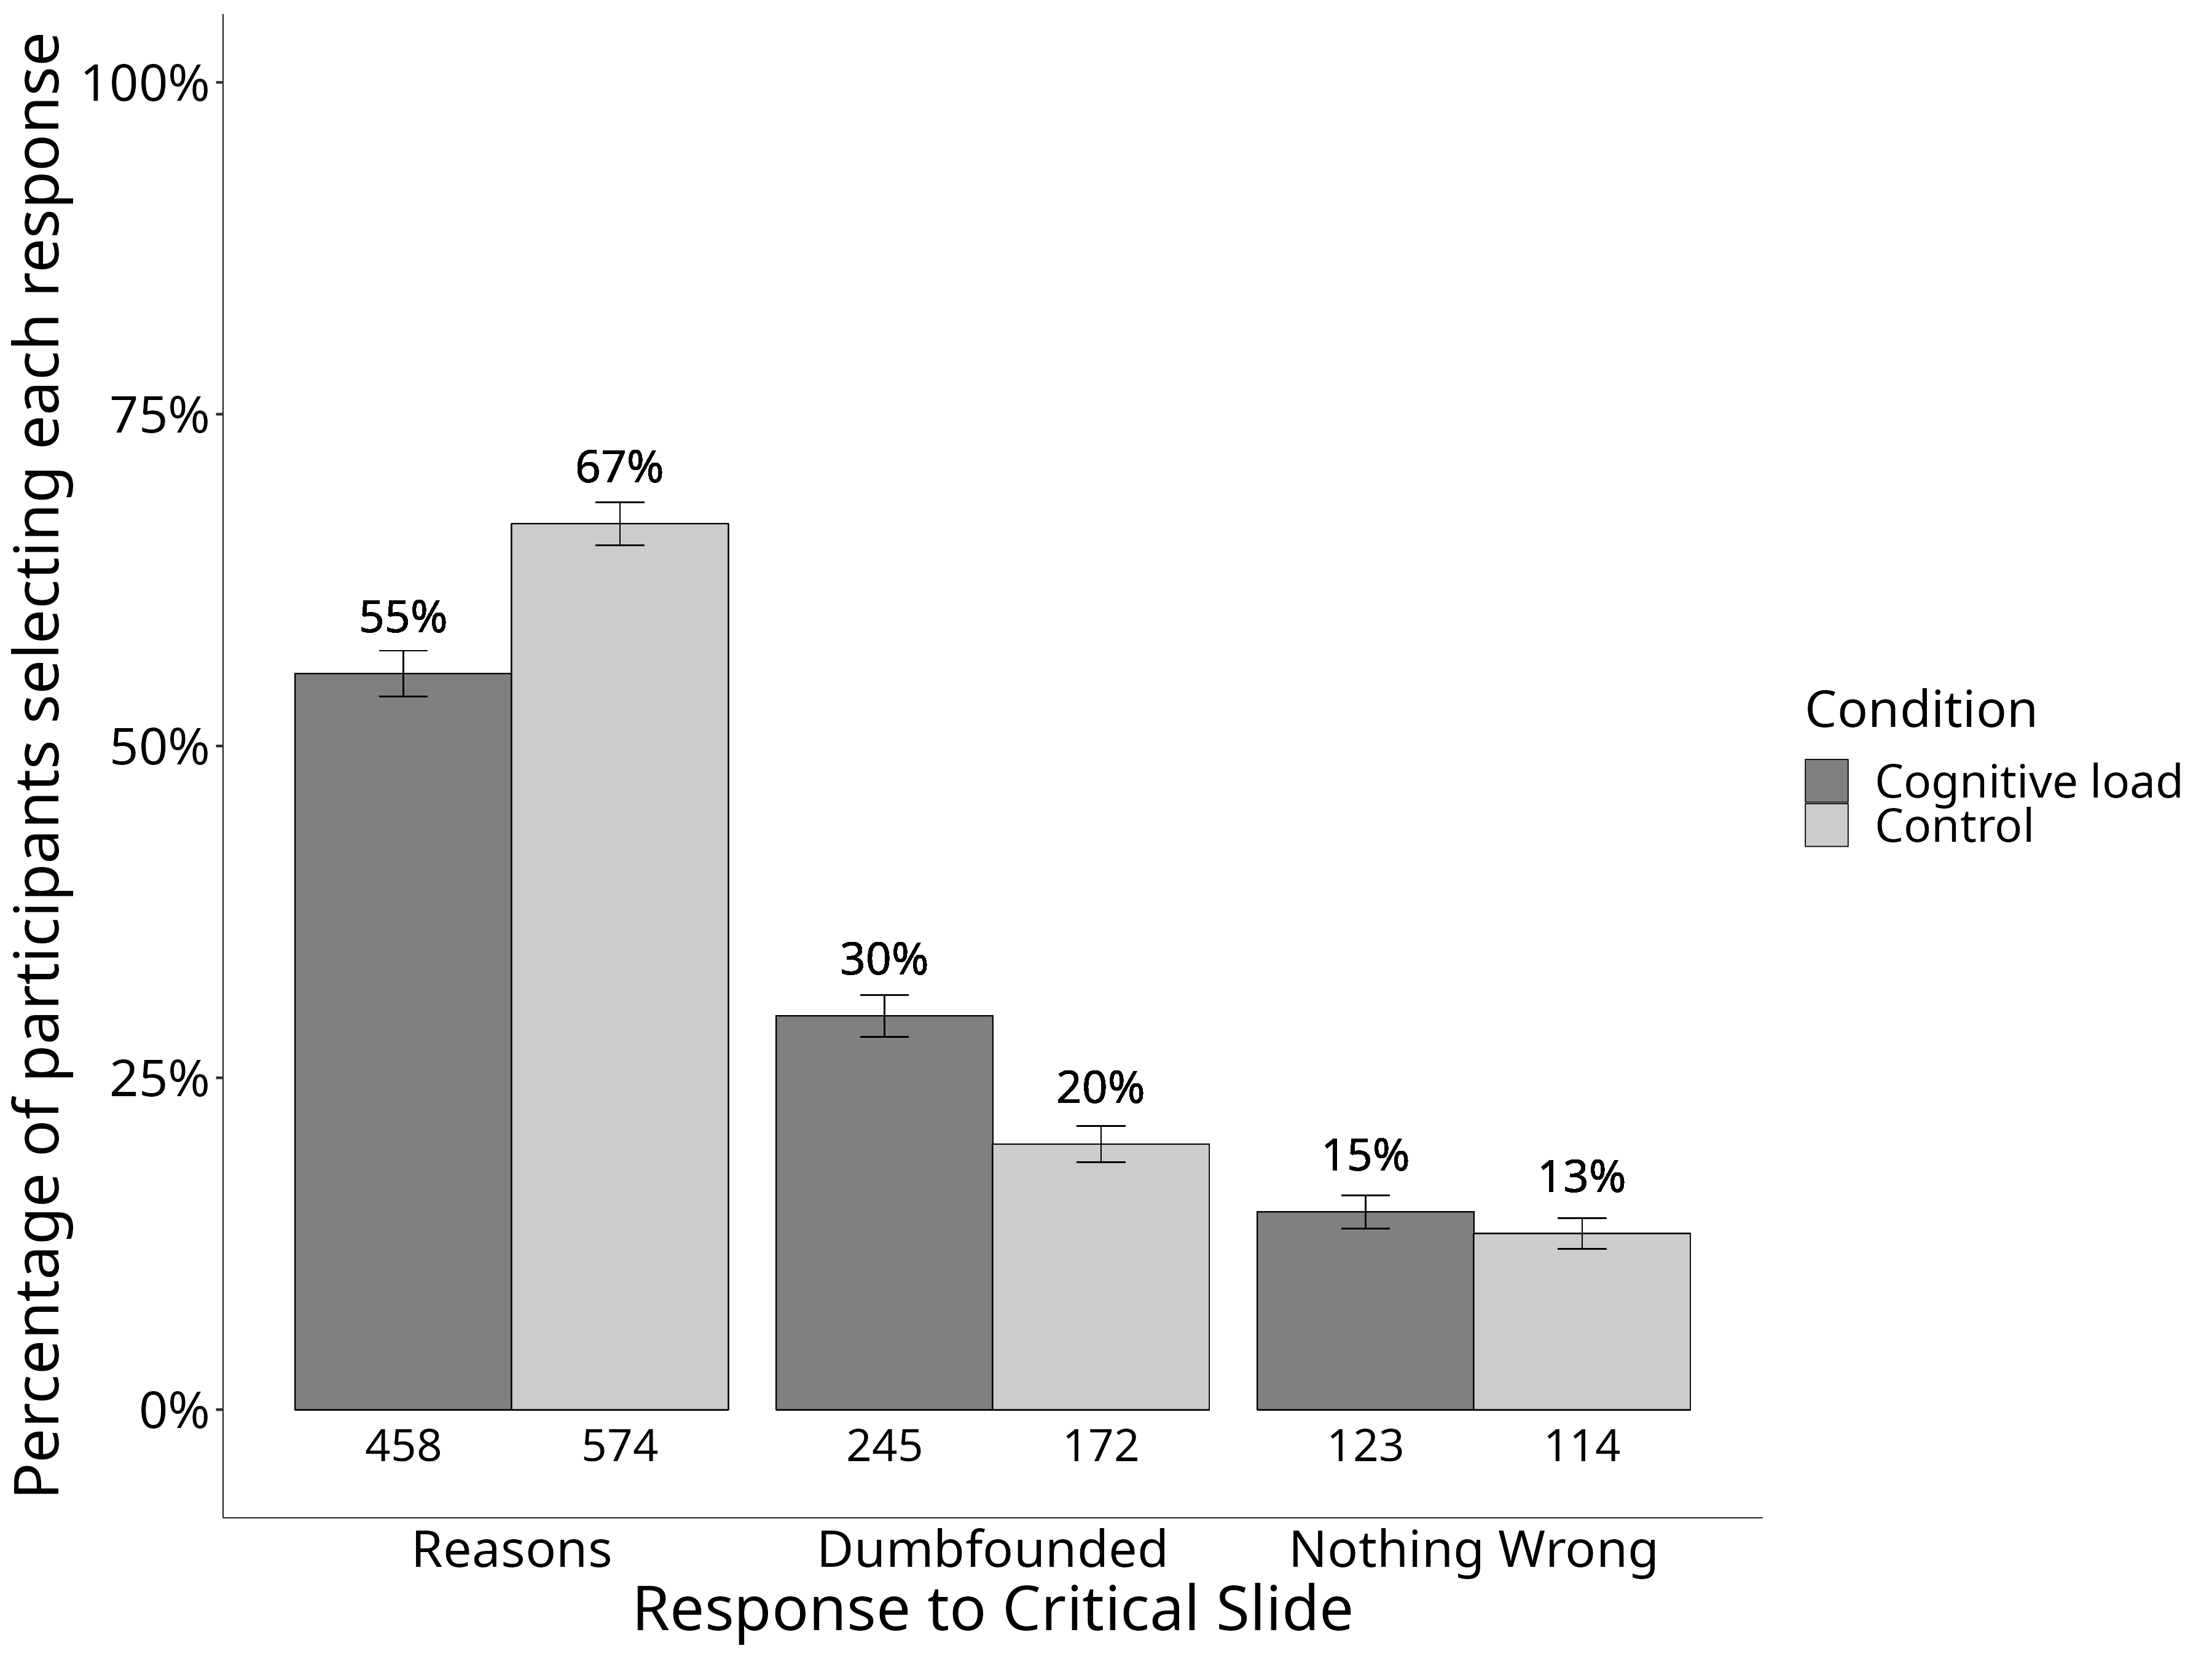
\includegraphics[width=6.25in,height=\textheight]{plots/overall.png}
\caption{Responses to critical slide depending on cognitive load}
\end{figure}

\begin{table}[tbp]

\begin{center}
\begin{threeparttable}

\caption{\label{tab:S6tab1dumb}Observed counts, expected counts, and standardised residuals for each response to the critical slide depending on cognitive load (full sample)}

\begin{tabular}{llcc}
\toprule
 & \multicolumn{1}{c}{} & \multicolumn{1}{c}{Cognitive Load} & \multicolumn{1}{c}{Control}\\
\midrule
Observed count & Reasons & 458 & 574\\
 & Dumbfounded & 245 & 172\\
 & Nothing Wrong & 123 & 114\\
Expected count & Reasons & 505.59 & 526.41\\
 & Dumbfounded & 204.3 & 212.7\\
 & Nothing Wrong & 116.11 & 120.89\\
Standardised residuals & Reasons & -4.76** & 4.76**\\
 & Dumbfounded & 4.6** & -4.6**\\
 & Nothing Wrong & 0.97 & -0.97\\
\bottomrule
\addlinespace
\end{tabular}

\begin{tablenotes}[para]
\normalsize{\textit{Note.} * = sig. at \emph{p} < .05; ** = sig. at \emph{p} < .001}
\end{tablenotes}

\end{threeparttable}
\end{center}

\end{table}

\newpage

This pattern was observed for all scenarios individually with the exception of \emph{Julie and Mark}, which showed no association between experimental condition and cognitive load, \(\chi\)\textsuperscript{2}(2, \emph{N} = 418) = 0.49, \emph{p} = .783, \emph{V} = 0.25, power = 0.601. The association was significant for \emph{Jennifer} \(\chi\)\textsuperscript{2}(2, \emph{N} = 418) = 17.33, \emph{p} \textless{} .001, \emph{V} = 0.24, power = 0.623, \emph{Trolley} \(\chi\)\textsuperscript{2}(2, \emph{N} = 418) = 10.95, \emph{p} = .004, \emph{V} = 0.25, power = 0.614, and Heinz, \(\chi\)\textsuperscript{2}(2, \emph{N} = 418) = 7.16, \emph{p} = .028, \emph{V} = 0.25, power = 0.608, see Figure~\ref{fig:S6ch5S6fig2criticalconditionb}. Supplementary Tables 20-23 show the direction of the effect for each scenario. Under cognitive load, fewer participants provided reasons and more participants provided a dumbfounded response for \emph{Jennifer}, \emph{Trolley}, and \emph{Heinz}

\begin{figure}
\centering
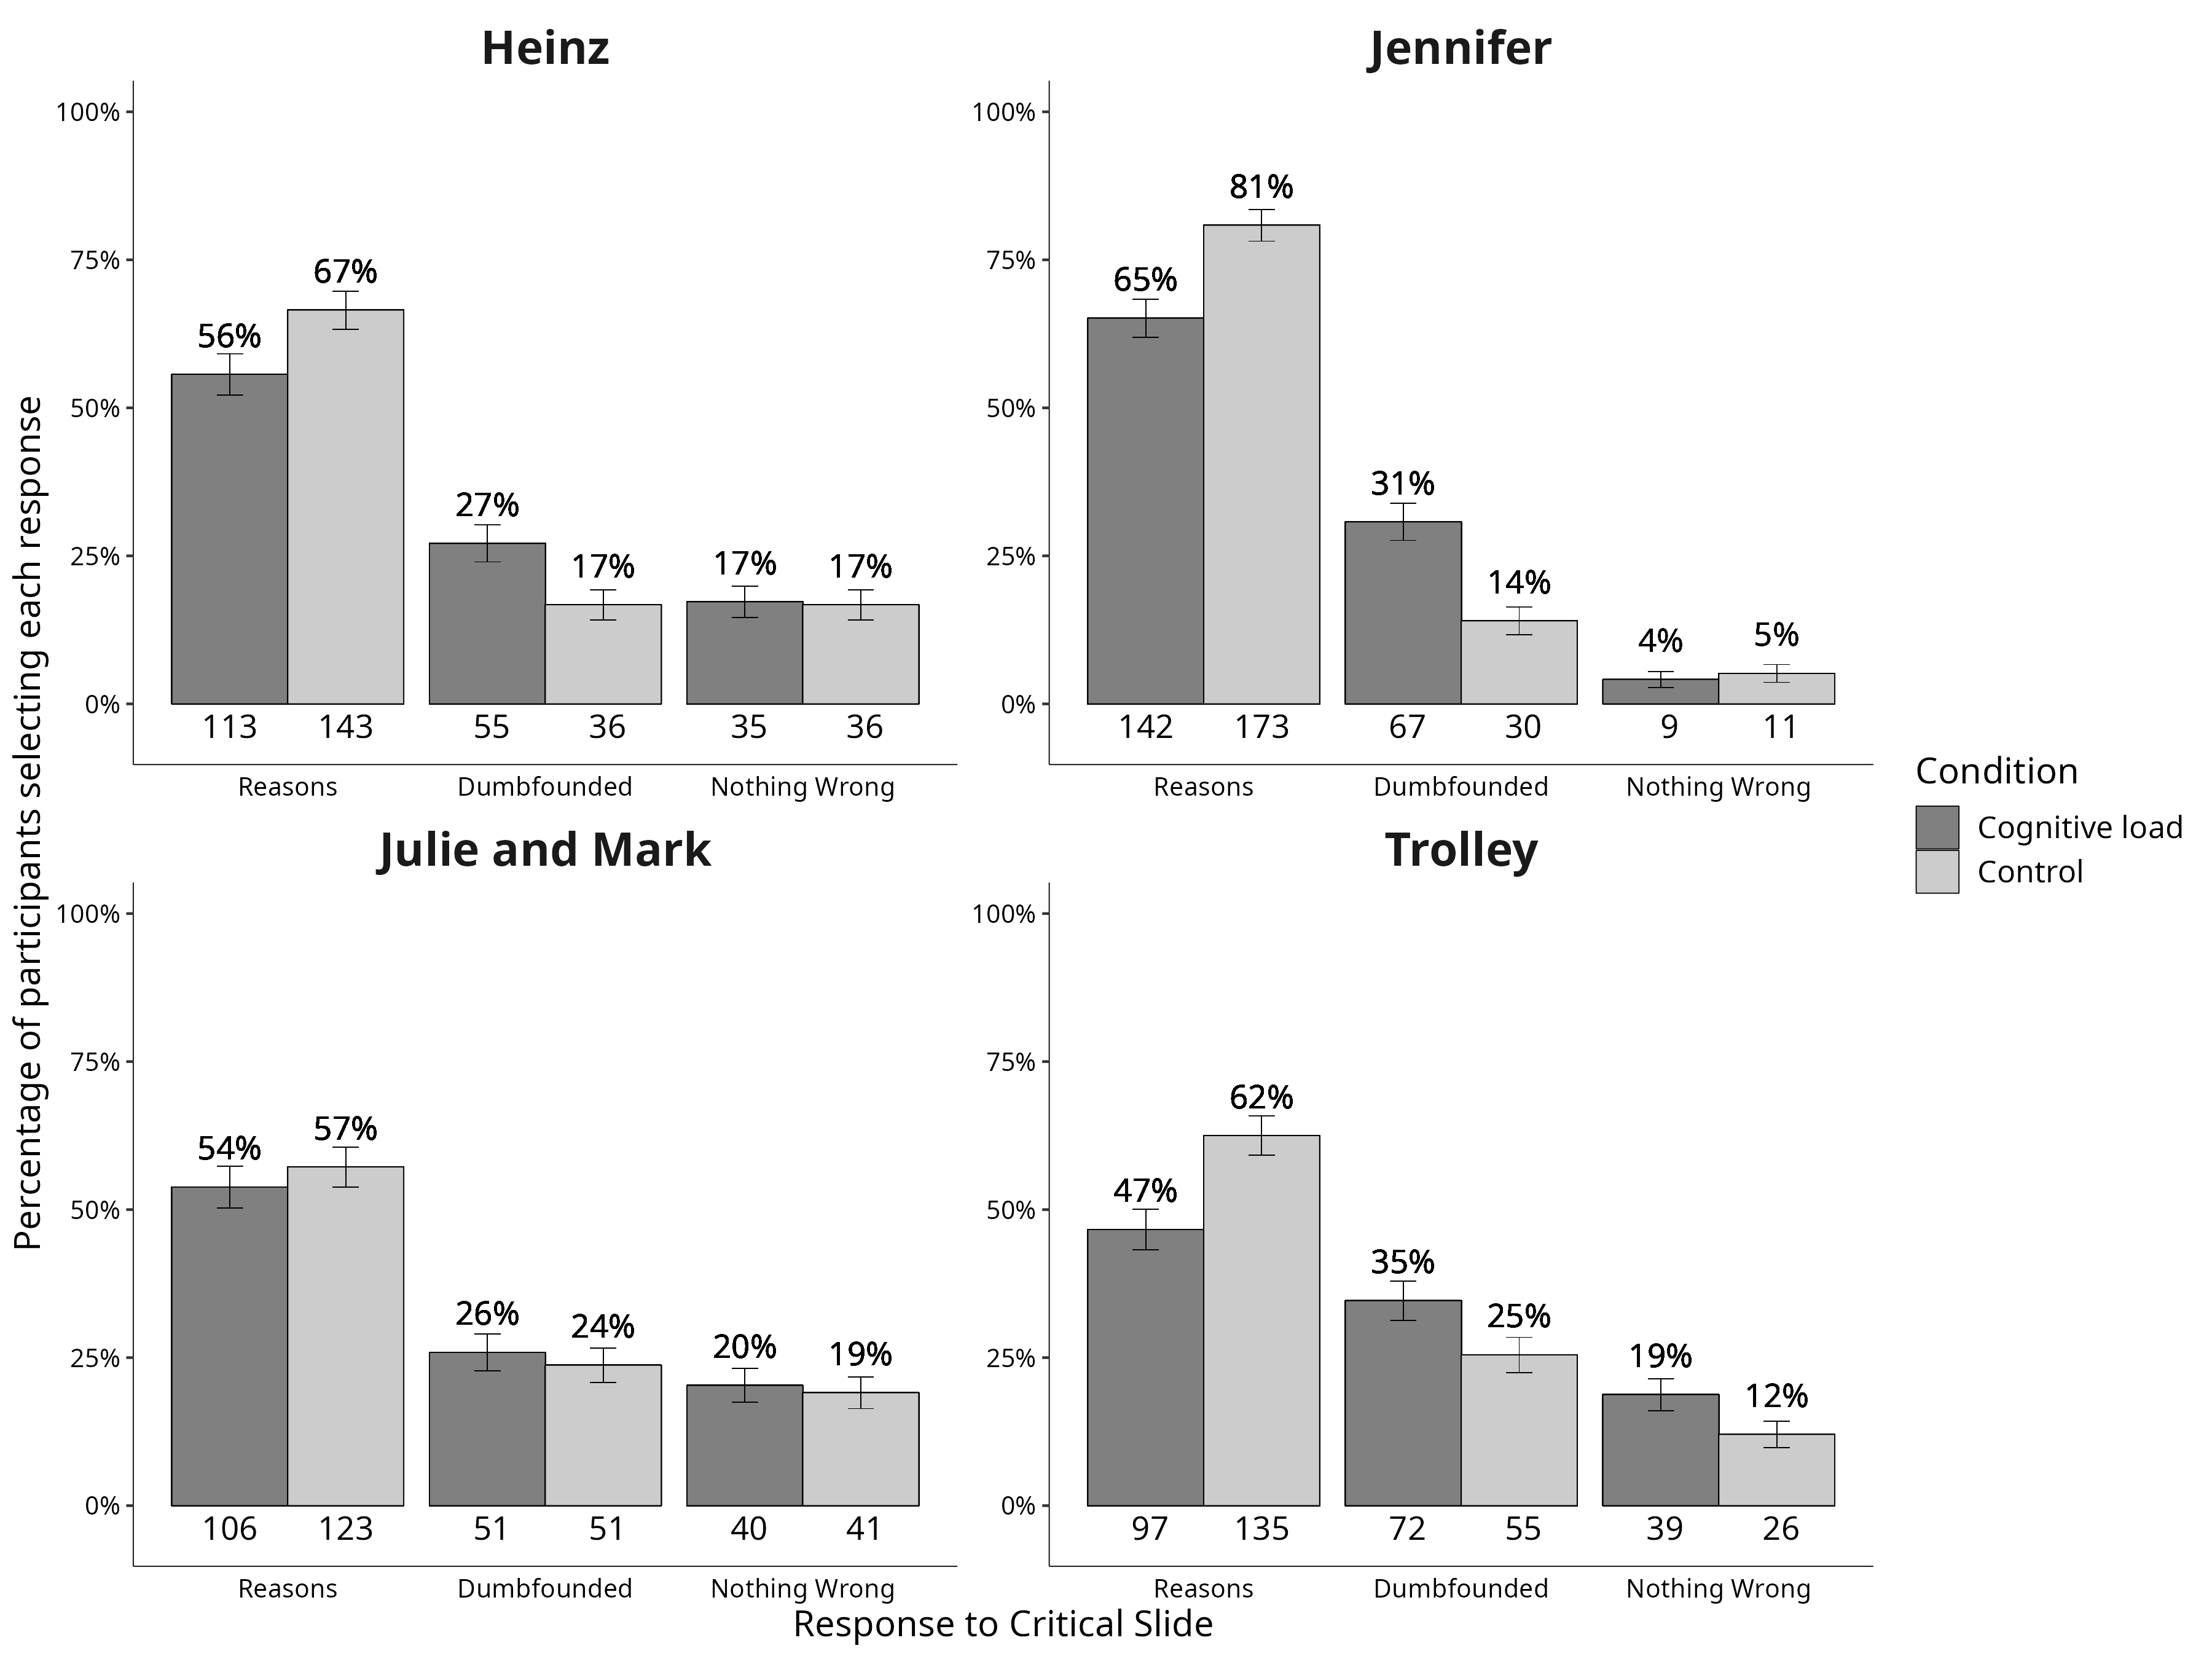
\includegraphics[width=6.25in,height=\textheight]{plots/all_scenarios.png}
\caption{Responses to critical slide and for the experimental group and the control group for each scenario}
\end{figure}

A chi-squared test for independence revealed a significant association between scenario and response to the critical slide, \(\chi\)\textsuperscript{2}(6, \emph{N} = 1686) = 61.34, \emph{p} \textless{} .001, \emph{V} = 0.19, the observed power was 1. Participants were significantly more likely to select ``There is nothing wrong'' for \emph{Julie and Mark} (\emph{p} = .002), more likely to provide reasons (\emph{p} = .002) and less likely to select ``There is nothing wrong'' (\emph{p} \textless{} .001) for Jennifer, and more likely to be dumbfounded by \emph{Trolley} (\emph{p} = .031).

A multinomial logistic regression was conducted to test the effects of cognitive load and scenario on dumbfounded responding. Overall the model was significant, \(\chi\)\textsuperscript{2}(8, \emph{N} = 1686) = 95.9, \emph{p} \textless{} .001, and explained between 6.07\% (Cox and Snell R square) and 7.22\% (Nadelkerke R squared) of the variance in responses to the critical slide, the observed power was 1. Participants in the control condition were significantly less likely to provide a dumbfounded response than to provide reasons, Wald = 25.04, \emph{p} \textless{} .001, \emph{OR} = 0.55, 95\% CI {[}0.44, 0.70{]}, in addition, participants in the control condition were also signifcantly less likely to select ``There is nothing wrong'', than to provide reasons, Wald = 5.23, \emph{p} = .022, \emph{OR} = 0.71, 95\% CI {[}0.54, 0.95{]}. For \emph{Jennifer}, participants were significantly less likely to select ``There is nothing wrong'' than to provide a reason, Wald = 30.87, \emph{p} \textless{} .001, \emph{OR} = 0.23, 95\% CI {[}0.13, 0.38{]}; while for \emph{Trolley} participants were significantly more likely to present as dumbfounded than to provide a reason, Wald = 6.89, \emph{p} = .009, \emph{OR} = 1.55, 95\% CI {[}1.12, 2.14{]}.

\hypertarget{refs}{}
\begin{CSLReferences}{1}{0}
\leavevmode\vadjust pre{\hypertarget{ref-greene_cognitive_2008}{}}%
Greene, J. D., Morelli, S. A., Lowenberg, K., Nystrom, L. E., \& Cohen, J. D. (2008). Cognitive load selectively interferes with utilitarian moral judgment. \emph{Cognition}, \emph{107}(3), 1144--1154. \url{https://doi.org/10.1016/j.cognition.2007.11.004}

\leavevmode\vadjust pre{\hypertarget{ref-mchugh_searching_2017a}{}}%
McHugh, C., McGann, M., Igou, E. R., \& Kinsella, E. L. (2017). Searching for {Moral Dumbfounding}: {Identifying Measurable Indicators} of {Moral Dumbfounding}. \emph{Collabra: Psychology}, \emph{3}(1), 1--24. \url{https://doi.org/10.1525/collabra.79}

\leavevmode\vadjust pre{\hypertarget{ref-r_core_team_r:_2021}{}}%
R Core Team. (2021). \emph{R: {A} language and environment for statistical computing} {[}Manual{]}. {Vienna, Austria}: {R Foundation for Statistical Computing}.

\end{CSLReferences}


\end{document}
